%%%%%%%%%%%%%%%%%%%%%%%%%%%%%%%%%%%%%%%%%
% Programming/Coding Assignment
% LaTeX Template
%
% This template has been downloaded from:
% http://www.latextemplates.com
%
% Original author:
% Ted Pavlic (http://www.tedpavlic.com)
%
% Note:
% The \lipsum[#] commands throughout this template generate dummy text
% to fill the template out. These commands should all be removed when 
% writing assignment content.
%
% This template uses a Perl script as an example snippet of code, most other
% languages are also usable. Configure them in the "CODE INCLUSION 
% CONFIGURATION" section.
%
%%%%%%%%%%%%%%%%%%%%%%%%%%%%%%%%%%%%%%%%%

%----------------------------------------------------------------------------------------
%	PACKAGES AND OTHER DOCUMENT CONFIGURATIONS
%----------------------------------------------------------------------------------------

\documentclass{article}
\usepackage[utf8]{inputenc}
\usepackage[brazil]{babel}

\usepackage{amsmath,amsthm,amssymb,amsfonts} % Math stuff
%\usepackage{enumitem,tikz}
\usepackage{enumitem} % Better enumerates

\usepackage{fancyhdr} % Required for custom headers
\usepackage{lastpage} % Required to determine the last page for the footer
\usepackage{extramarks} % Required for headers and footers
\usepackage[usenames,dvipsnames]{color} % Required for custom colors
\usepackage{graphicx} % Required to insert images
\usepackage{listings} % Required for insertion of code
\usepackage{courier} % Required for the courier font
\usepackage{lipsum} % Used for inserting dummy 'Lorem ipsum' text into the template

% Margins
\topmargin=-0.45in
\evensidemargin=0in
\oddsidemargin=0in
\textwidth=6.5in
\textheight=9.0in
\headsep=0.25in

\linespread{1.1} % Line spacing

% Set up the header and footer
\pagestyle{fancy}
\lhead{\hmwkClass: \hmwkTitle} % Top left head
\chead{} % Top center head
%\rhead{\firstxmark} % Top right header
\lfoot{\lastxmark} % Bottom left footer
\cfoot{} % Bottom center footer
\rfoot{Página\ \thepage\ de\ \protect\pageref{LastPage}} % Bottom right footer
\renewcommand\headrulewidth{0.4pt} % Size of the header rule
\renewcommand\footrulewidth{0.4pt} % Size of the footer rule

\setlength\parindent{0pt} % Removes all indentation from paragraphs

%----------------------------------------------------------------------------------------
%	DOCUMENT STRUCTURE COMMANDS
%	Skip this unless you know what you're doing
%----------------------------------------------------------------------------------------

% Header and footer for when a page split occurs within a problem environment
\newcommand{\enterProblemHeader}[1]{
\nobreak\extramarks{#1}{#1 continued on next page\ldots}\nobreak
\nobreak\extramarks{#1 (continued)}{#1 continued on next page\ldots}\nobreak
}

% Header and footer for when a page split occurs between problem environments
\newcommand{\exitProblemHeader}[1]{
\nobreak\extramarks{#1 (continued)}{#1 continued on next page\ldots}\nobreak
\nobreak\extramarks{#1}{}\nobreak
}

\setcounter{secnumdepth}{0} % Removes default section numbers
\newcounter{homeworkProblemCounter} % Creates a counter to keep track of the number of problems

\newcommand{\homeworkProblemName}{}
\newenvironment{homeworkProblem}[1][\unskip]{ % Sets homework environment with adittional argument for extra naming
    \stepcounter{homeworkProblemCounter} % Increase counter for number of problems
    \renewcommand{\homeworkProblemName}{Questão \arabic{homeworkProblemCounter} #1} % Assign \homeworkProblemName the name of the problem
    \subsection{\homeworkProblemName} % Make a section in the document with the custom problem count
    \enterProblemHeader{\homeworkProblemName} % Header and footer within the environment
}{
\exitProblemHeader{\homeworkProblemName} % Header and footer after the environment
}

\newcommand{\problemAnswer}[1]{ % Defines the problem answer command with the content as the only argument
\noindent\framebox[\columnwidth][c]{\begin{minipage}{0.98\columnwidth}#1\end{minipage}} % Makes the box around the problem answer and puts the content inside
}

\newcommand{\homeworkSectionName}{}
\newenvironment{homeworkSection}[1]{ % New environment for sections within homework problems, takes 1 argument - the name of the section
\renewcommand{\homeworkSectionName}{#1} % Assign \homeworkSectionName to the name of the section from the environment argument
\subsection{\homeworkSectionName} % Make a subsection with the custom name of the subsection
\enterProblemHeader{\homeworkProblemName\ [\homeworkSectionName]} % Header and footer within the environment
}{
\enterProblemHeader{\homeworkProblemName} % Header and footer after the environment
}

%----------------------------------------------------------------------------------------
%	NAME AND CLASS SECTION
%----------------------------------------------------------------------------------------

\newcommand{\hmwkTitle}{Relatório EP 1} % Assignment title
\newcommand{\hmwkDueDate}{18 de Setembro de 2016} % Due date
\newcommand{\hmwkClass}{MAC0210} % Course/class

%----------------------------------------------------------------------------------------
%	TITLE PAGE
%----------------------------------------------------------------------------------------

\title{
\vspace{2in}
\textmd{\textbf{\hmwkClass:\ \hmwkTitle}}\\
\normalsize\vspace{0.1in}\small{\hmwkDueDate}\\
\vspace{3in}
}

\author{\textbf{Nathan Benedetto Proença - 8941276}\\
\textbf{Victor Sena Molero - 8941317}}
\date{} % Insert date here if you want it to appear below your name

%----------------------------------------------------------------------------------------

\begin{document}

\maketitle

%----------------------------------------------------------------------------------------
%	TABLE OF CONTENTS
%----------------------------------------------------------------------------------------

%\setcounter{tocdepth}{1} % Uncomment this line if you don't want subsections listed in the ToC

\newpage
\tableofcontents
\newpage

\section{Parte 1: Aritmética de Ponto Flutuante}

\begin{homeworkProblem}[(3.11)]
Suponha que temos um sistema de representação de ponto flutuante com base 2 e,  
$$x = \pm S \times 2^{E} \text{, }$$
$$\text{com }  S = (0.1b_2b_3b_4\dots b_{24}) \text{, } $$
$$\text{i.e, }  \frac{1}{2} \leq S < 1$$
onde o expoente $-128 < E < 127$.

\begin{enumerate}[label={\alph*)}]
    \item Qual é o maior número de ponto flutuante desse sistema?
        \begin{proof}[Resposta]
        $2^{126} - 2^{101}$, basta preencher todos os bits (de $b_2$ até $b_{24}$) e escolher o maior expoente possível.
        \end{proof}
    \item Qual é o menor número de ponto flutuante positivo desse sistema?
        \begin{proof}[Resposta]
        $2^{-128}$, basta escolher a menor mantissa possível ($0.1$) e o menor expoente possível ($-127$).
        \end{proof}
    \item Qual é o menor inteiro positivo que não é exatamente representável nesse sistema?
        \begin{proof}[Resposta]
        $2^{24} + 1$, basta escolher a menor mantissa não representável ($0.10\dots 01$) e o menor expoente para o qual ela representa um inteiro ($25$).
        \end{proof}
\end{enumerate}
\end{homeworkProblem}

\begin{homeworkProblem}[(5.1)]
Qual é a representação do número $1/10$ no formato IEEE single para cada um dos quatro modos de arredondamento?
\begin{proof}[Resposta]
A resposta curta é: 
$$x = 0.0\overline{0011} \text{, }$$
$$\mathrm{round\_down}(x) = \mathrm{round\_towards\_zero}(x) = 1.10011001100110011001100 \times 2^{-4} \text{ e }$$ 
$$\mathrm{round\_up}(x) = \mathrm{round\_to\_nearest}(x) = 1.10011001100110011001101 \times 2^{-4} \text{.}$$

Se $x$ é uma representação binária exata de $1/10$, $x = 0.0\overline{0011} = 1.\overline{1001} \times 2^{-4}$ (os números abaixo da barra representam uma dízima periódica, se repetem infinitamente).

Calculamos então $x_- = 1.10011001100110011001100 \times 2^{-4}$ e $x_+ = 1.10011001100110011001101 \times 2^{-4}$. Se o modo é \textit{Round Down}, o número será representado por $x_-$ e se for \textit{Round Up}, será $x_+$, ambos pela definição dos modos.

Já que $x > 0$, o modo $\textit{Round towards zero}$ também usará $x_-$, porém $x$ é mais próximo de $x_+$ do que de $x_-$, basta perceber que o erro relativo entre $x$ e $x_-$ é maior que $1/2$, portanto, o modo $\textit{Round to nearest}$ usará a representação $x_+$.
\end{proof}
E para os números $1 + 2^{-25}$
\begin{proof}[Resposta]
$$x = 1.0000000000000000000000001 \times 2^0\text{, }$$
$$\mathrm{round\_down}(x) = \mathrm{round\_towards\_zero}(x) = \mathrm{round\_to\_nearest}(x) = 1.00000000000000000000000 \times 2^0\text{, }$$
$$\mathrm{round\_up}(x) = 1.00000000000000000000001 \times 2^0\text{.}$$
Se $x$ é uma representação binária exata de $1+2^{-25}$, $x = 1.0000000000000000000000001 \times 2^0$, $x_- = 1.00000000000000000000000 \times 2^0$ e $x_+ = 1.00000000000000000000001 \times 2^0$. O modo \textit{Round down} vai levar para $x_-$ e o modo \textit{Round up} vai levar para $x_+$, como sempre.  

Já que $x > 0$, o modo $\textit{Round towards zero}$ também usará $x_-$, além disso, o erro relativo entre $x$ e $x_-$ é $1/4$, logo, o modo $\textit{Round to nearest}$ também levará para $x_-$.
\end{proof}
e $2^{130}$?
\begin{proof}[Resposta]
$$x = 1 \times 2^{130} \text{, }$$
\begin{equation*} \begin{split}
    \mathrm{round\_down}(x) = \mathrm{round\_towards\_zero}(x) = \mathrm{round\_to\_nearest}(x) = \\
    = \mathrm{round\_up}(x) = 1.00000000000000000000000 \times 2^{130}\text{.}
\end{split} \end{equation*}
Se $x$ é uma representação binária exata de $2^{130}$, $x = 1 \times 2^{130}$, porém, $x$ é exatamente representável no sistema IEEE single, logo, em todos os modos de arredondamento, será representado como $1.00000000000000000000000 \times 2^{130}$.
\end{proof}
\end{homeworkProblem}

\begin{homeworkProblem}[(6.4)]
Qual é o maior número de ponto flutuante $x$ tal que $1 \oplus x$ é exatamente 1, assumindo que o formato usado é IEEE single e modo de arredondamento para o mais próximo?

\begin{proof}[Resposta]
$x = 2^{-24}$. $1 + x$ é igualmente próximo de $1 + 2^{-23}$ e $1$, porém, por causa do critério de arredondamento em empate (0 menos significativo), ele é arredondado para $1$, qualquer $x$ maior do que esse causará um arredondamento para um número maior do que $1$.
\end{proof}

E se o formato for IEEE double?

\begin{proof}[Resposta]
$x = 2^{-53}$, seguindo a mesma lógica usada para concluir a resposta do item anterior.
\end{proof}
\end{homeworkProblem}

\begin{homeworkProblem}[(6.8)]
Em aritmética exata, a soma é um operador comutativo e associativo. O operador de soma de ponto flutuante é comutativo?

\begin{proof}[Resposta]
Sim, pois para calcular o resultado em soma de ponto flutuante o padrão exige que seja calculado o valor exato e, então, arredondado para o sistema escolhido. Formalmente, denotaremos por $fl(x)$ a representação em ponto flutuante de um real $x$ e por $\oplus$ a operação de soma em ponto flutuante. Temos $fl(x) \oplus fl(y) = fl(fl(x) + fl(y)) = fl(fl(y) + fl(x)) = fl(y) \oplus fl(x)$.
\end{proof}

E associativo?

\begin{proof}[Resposta]
Não, os erros de arredondamento podem fazer com que a ordem das somas faça diferença. Por exemplo, considere um sistema com um dígito binário de precisão ($1.b_1$) e expoentes entre $-4$ e $4$, por exemplo. Escolha os números $x = 1 = 2^0$ e $y = z = 1/4 = 2^{-2}$. Teremos, na notação do sistema (base binária) que $(x \oplus y) \oplus z = (1.0 \times 2^0 \oplus 1.0 \times 2^{-2}) \oplus 1.0 \times 2^{-2} = 1.0 \times 2^0 \oplus 1.0 \times 2^{-2} = 1.0 \times 2^0$, por outro lado, $x \oplus (y \oplus z) = 1.0 \times 2^0 \oplus 1.0 \times 2^{-1} = 1.1 \times 2^0$.
\end{proof}
\end{homeworkProblem}

\section{Parte 2: Bacias de Newton}
Para se obter as bacias é necessário aplicar o método de Newton nos $n^2$ pontos do grid criado no plano complexo. Isso ocorre devido à restrição das funções que deveriam ser implementadas descritas no enunciado. Tivesse as iteraçoes do método acesso aos pontos já calculados, poderia se aproveitar desta informação e ter uma implementação muito mais eficiente.  

Assim, o que buscamos foi otimizar as iterações do método de Newton. Dado que os pontos iniciais e a função são quem ditam a taxa de convergência do método, e, além disto, estão fixados pela instância do problema, nossos esforços para melhorar a performance se tornaram mais restritos ainda e consistem em usufruir das vantagens da vetorização em \textsc{Matlab}.  

Felizmente, tanto a avaliação do polinõmio em um ponto quanto a derivação dele são operadores lineares. Isso nos permitiu expressar ambos de forma sucienta. A avaliação se reduz a um produto interno com um vetor cuja $i$-ésima coordenada é $x^{n-1-i}$ e a derivação é o resultado de aplicar uma matriz diagonal no vetor de coeficientes, que em \textsc{Matlab} pode facilmente ser implementado através de um produto componente a componente entre os vetores.

Outro fator que impactou bstante a eficiência do código foi o tratamento de entrada e saída. O comportamento padrão da função \textsc{fprintf} é de limpar o buffer de saída a cada chamada da função. Isso causou um grande \textit{overhead} no programa, pois eram adicionados poucos caracteres a cada chamada desta função, o que faz a chamada acontecer várias vezes para que toda a saída seja impressa. Assim, houve notória melhoria ao mudar a flag passada à função \textsc{fopen} para que o buffer de saída fosse descarregado apenas ao final do programa.

\subsection{Exemplos}

Para ilustrar o uso do método desenvolvido na parte 3 do EP. Escolhemos gerar as \textit{Newton Basins} para um polinômio e as expansões de Taylor deste polinômio em torno do ponto 0. Para isso, escolhemos a função $f(x) = x^6 + (3-7i)x^5 + (-20-15i)x^4 + (-40+20i)x^3 + (-26+40i)x^2 + (52+52i)x$ e rodamos nosso EP nela.  
\begin{center}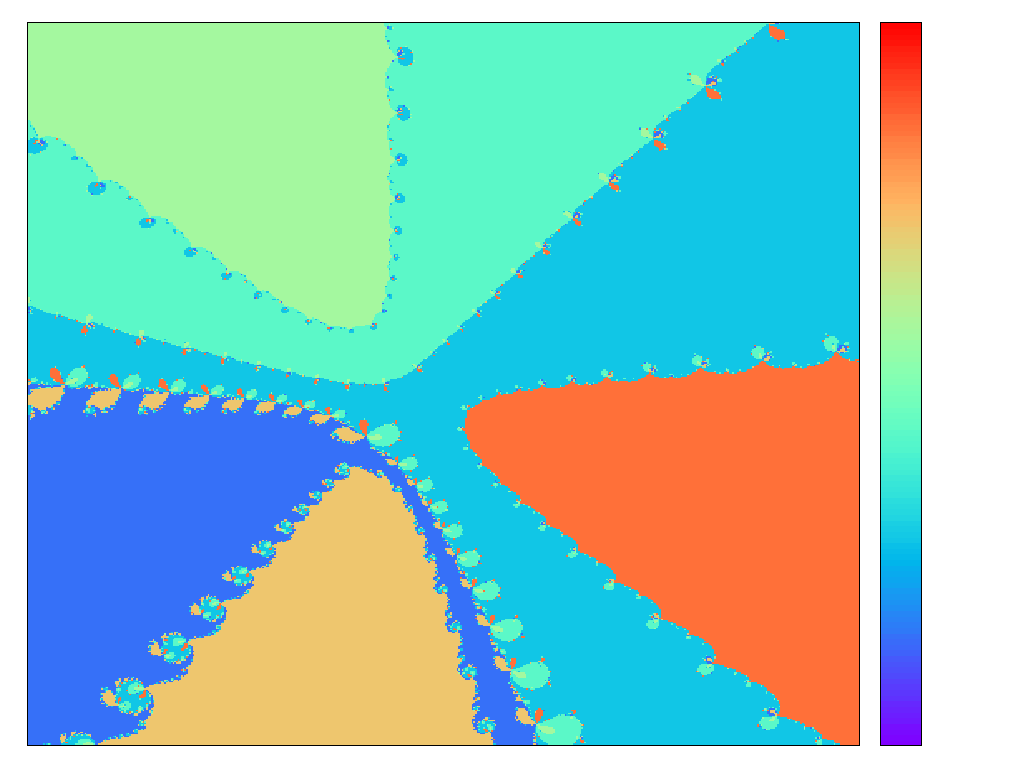
\includegraphics[width=0.75\columnwidth]{original} \end{center}
E, como planejado, repetimos o processo para as expansões de Taylor de diversos graus deste polinômio. Denotaremos a $i$-ésima expansão por $f_i(x)$. Primeiro, expandimos em grau 1, ou seja $f_1(x) = (52+52i)x$.  
\begin{center}
\includegraphics[width=0.75\columnwidth]{expand_1} \end{center}
Seguido de $f_2(x) = (-26+40i)x^2 + (52+52i)x$.  
\begin{center}
\includegraphics[width=0.75\columnwidth]{expand_2} \end{center}
Depois $f_3(x) = (-40+20i)x^3 + (-26+40i)x^2 + (52+52i)x$.  
\begin{center}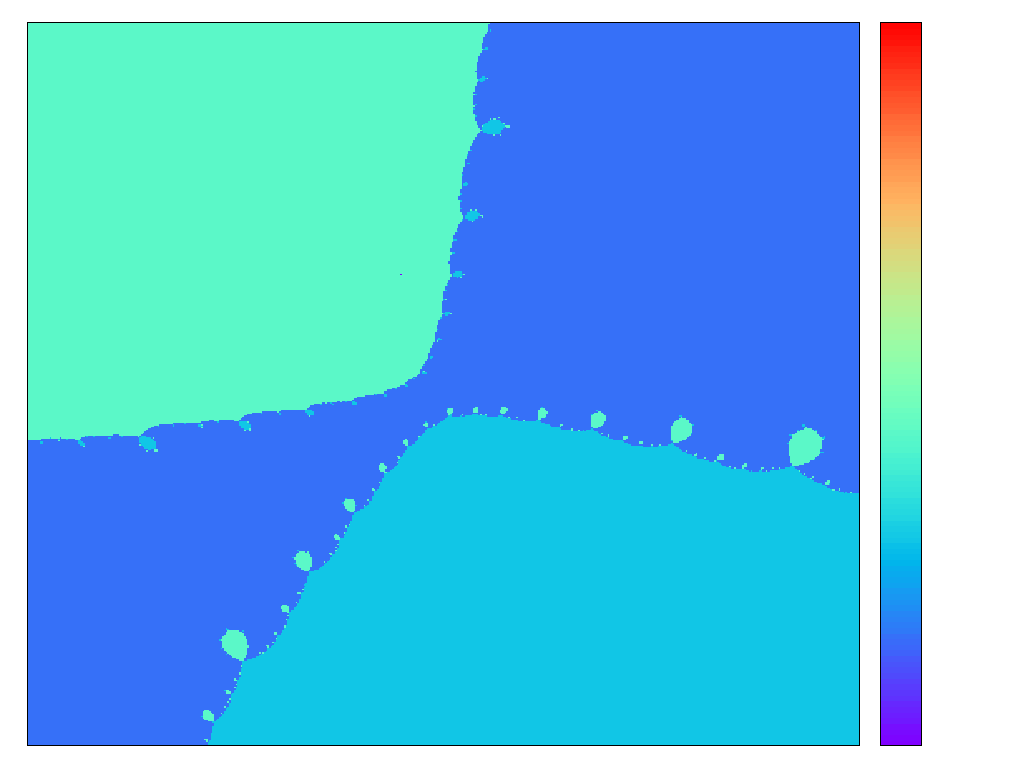
\includegraphics[width=0.75\columnwidth]{expand_3} \end{center}
Depois $f_4(x) = (-20-15i)x^4 + (-40+20i)x^3 + (-26+40i)x^2 + (52+52i)x$.  
\begin{center}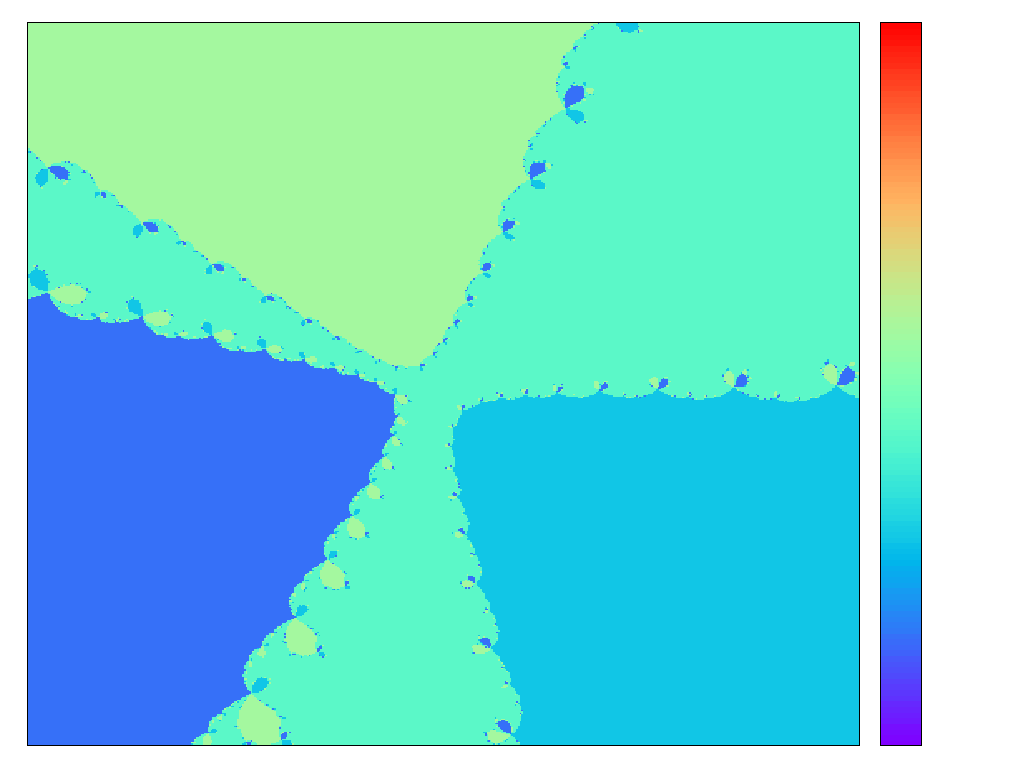
\includegraphics[width=0.75\columnwidth]{expand_4} \end{center}
E, finalmente, $f_5(x) = (3-7i)x^5 + (-20-15i)x^4 + (-40+20i)x^3 + (-26+40i)x^2 + (52+52i)x$.  
\begin{center}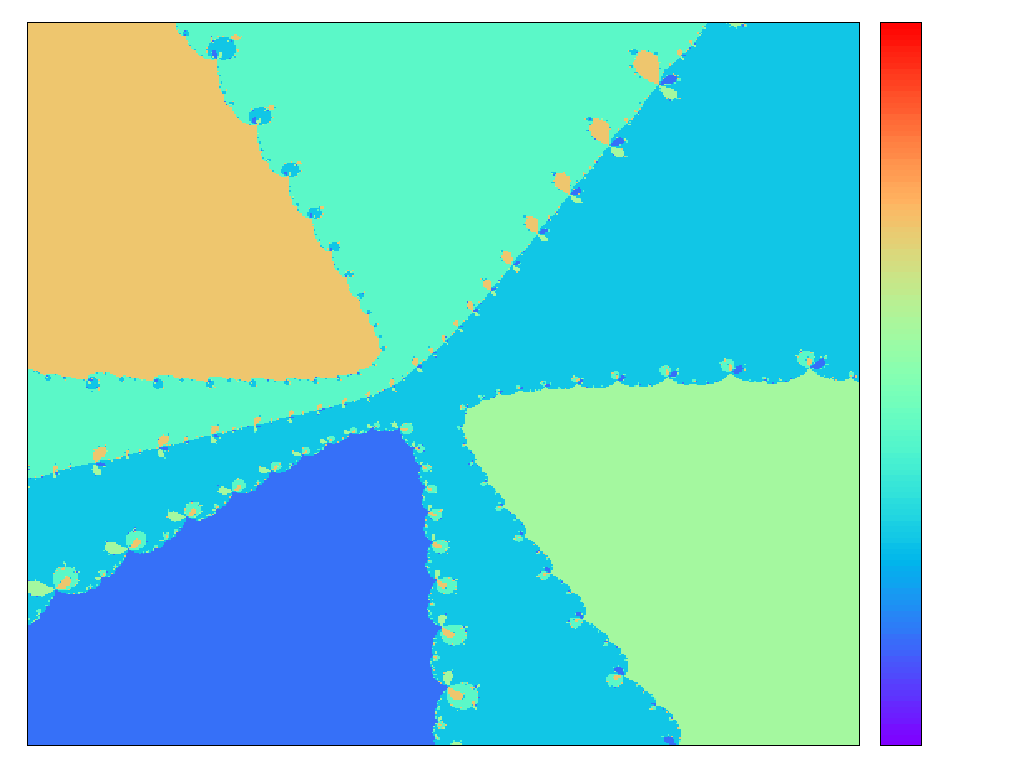
\includegraphics[width=0.75\columnwidth]{expand_5} \end{center}

\section{Parte 3: Encontrando todas as raízes de funções}
Novamente aqui há poucas decisões de projeto a serem feitas. O enunciado já descreve o algoritmo e os critérios para as decisões, restando pouco a ser feito que não implementar.  

Assumimos que as funções anônimas eram vetorizadas, para que pudessem ser facilmente aplicadas em diversos pontos. Além disso, utilizamos o método descrito apenas nos intervalos nos quais nenhuma das bordas era uma raíz da função. Isso descarta possíveis pontos, mas interpretamos como uma limitação do método em si, por ser sensível à escolha do $\textit{ninter}$.  

O que é uma solução simples para tratar o caso em que raízes da função estão entre os pontos da primeira amostragem é retornar a união das raízes encontradas ao se chamar com $\textit{ninter}$ e $\textit{ninter} + 1$.  

Isto resolve pois é impossível que um valor de $x$ seja borda de intervalos em ambos os casos. Se fosse, existiriam inteirom $0 \leq k \leq n$ e $0 \leq t \leq n+1$ tais que
$$ a + k*(b-a)/n = a + t(b-a)/(n+1) \text{, ou seja,}$$
$$(n+1)k = nt$$
Mas este inteiro $(n+1)k$, por ser múltiplo de $n$, é um múltiplo de $\mathrm{mmc}(n+1,n) = n(n+1)$. Mas isso implica que $k \geq n$, o que nos permite afirmar que este ponto em comum é o próprio $b$. Assim, tratamos todos os possíveis pontos que são raíz no interior do intervalo, sem piora na complexidade.  

O método se mostrou robusto, encontrando todas as raízes de ambas verificações dadas no enunciado. Para testar, pode-se abrir o \textit{octave} na pasta 03 e rodar 
\begin{equation*} \begin{split}
    \texttt{find\_all\_roots(@(t)(sinc(t./pi),} \\
    \texttt{@(t)(t.*cos(t)-sin(t))./(t.*t)),} \\
    \texttt{-10, 10, 10**(-5), 100)}
\end{split} \end{equation*}.
\end{document}

